\documentclass[a4paper,12pt]{report}
\usepackage[utf8]{inputenc}
%\usepackage[frenchb]{babel}
\usepackage[T1]{fontenc}
\usepackage{lmodern,textcomp}
\usepackage{graphicx}
%\usepackage{listings}
\usepackage{caption}
%\usepackage{fancybox}
\usepackage[pdftex]{hyperref}
%\usepackage{epsfig}
\usepackage{fancyvrb}
\usepackage{tikz}
\usetikzlibrary{shapes.geometric,backgrounds,fit,positioning,trees}
\usetikzlibrary{shapes.callouts}
%\usetikzlibrary{arrows.meta,shapes.callouts}
\usepackage{wrapfig}
\usepackage{manfnt}
\usepackage{dingbat}
\usepackage{xcolor}
\usepackage{geometry}

\definecolor{reddebian}{rgb}{0.84314,0.03922,0.32549}
\definecolor{bluedane}{rgb}{0.09020,0.56863,1}
\definecolor{greendane}{rgb}{0.43137,0.60784,0.14510}
\def\purpledane{violet}

\hypersetup{%
  pdftitle={Xia},
  pdfauthor={Énuma Logiciel Libre},
  pdfsubject={Xia},
  pdfkeywords={Xia, logiciel libre, html5, Inkscape},
  colorlinks= true,
  linkcolor = greendane,
  urlcolor = bluedane
  }

% La dimension des marges
\geometry{hscale=0.7,vscale=0.7}

\title{Xia\\ Create HTML5 "images-actives"}

\renewcommand{\thechapter}{\arabic{chapter}}
\renewcommand{\thesection}{\Roman{section}}
\renewcommand{\thesubsection}{\alph{subsection}}

% pour unifier les indications relatives aux manipulation à effectuer dans les logiciels
% à modifier au besoin
\newcommand{\chemin}[1]{\texttt{\textcolor{reddebian}{#1}}}

% L'environnement alerte                        
\newsavebox{\boiteBrouillon}
\newcommand{\virageDanger}{\textdbend}

\newlength{\LargeurBouleAlerte}
\settowidth{\LargeurBouleAlerte}{%
  
\begin{tikzpicture}%
    \node{\virageDanger};%
  \end{tikzpicture}%
}

% Style pour la boîte alerte
\tikzstyle{boitealerte}=[draw=red,rounded corners,inner xsep=1em,inner ysep=1ex]

% Style pour la boule alerte
\tikzstyle{boulealerte}=[circle,ball color=red,text=white] 

\newenvironment{alerte}{%
  \begin{lrbox}{\boiteBrouillon}% On sauve dans \boiteBrouillon le contenu
    \begin{minipage}{.8\linewidth}%  
      \color{red}%
      \setlength{\parskip}{1ex plus 0.2ex minus 0.2ex}%
}{%
    \end{minipage}%
  \end{lrbox}% Fin. Attention lrbox stocke du contenu sur 1 ligne (pas de paragrpahe)
  % La boîte peut être utilisée via \usebox{\boiteBrouillon}
  \vspace{1.5ex}%
  
\begin{tikzpicture}%
    \node [boitealerte] (cadre) {%
      \hspace{0.5\LargeurBouleAlerte}%
      \usebox{\boiteBrouillon}%
    };%
    \node [boulealerte] (alerte) at (cadre.west) {\virageDanger};%
  \end{tikzpicture}%
  \vspace{1.5ex}%
}        

% L'environnement astuce
\newcommand{\pouceOK}{\large\leftthumbsup}

\newlength{\LargeurBouleAstuce}
\settowidth{\LargeurBouleAstuce}{%
  \begin{tikzpicture}%
    \node{\pouceOK};%
  \end{tikzpicture}%
}

\tikzstyle{bouleastuce}=[circle,ball color=teal,text=white]

\tikzstyle{boiteastuce}=[draw=teal,rounded corners,inner xsep=1em,inner ysep=1ex]
                        
\newenvironment{astuce}{%
  \begin{lrbox}{\boiteBrouillon}% On sauve dans \boiteBrouillon le contenu
    \begin{minipage}{.8\linewidth}%
      \color{teal}%
      \setlength{\parskip}{1ex plus 0.2ex minus 0.2ex}%
}{%
    \end{minipage}%
  \end{lrbox}% Fin. Attention lrbox stocke du contenu sur 1 ligne (pas de paragrpahe)
  % La boîte peut être utilisée via \usebox{\boiteBrouillon}
  \vspace{1.5ex}%
  
\begin{tikzpicture}%
    \node [boiteastuce] (cadre) {%
      \hspace{0.5\LargeurBouleAstuce}%
      \usebox{\boiteBrouillon}%
    };%
    \node [bouleastuce] (astuce) at (cadre.west) {\pouceOK};%
  \end{tikzpicture}%
  \vspace{1.5ex}%
}    

% L'environnement links
\newcommand{\mainDroite}{\large\leftpointright}

\newlength{\LargeurBouleLinks}
\settowidth{\LargeurBouleLinks}{%
  \begin{tikzpicture}%
    \node{\mainDroite};%
  \end{tikzpicture}%
}

\tikzstyle{boulelinks}=[circle,ball color=\purpledane,text=white]

\tikzstyle{boitelinks}=[draw=\purpledane,rounded corners,inner xsep=1em,inner ysep=1ex, align=right]
                        
\newenvironment{links}{%
  \begin{lrbox}{\boiteBrouillon}% On sauve dans \boiteBrouillon le contenu
    \begin{minipage}{.8\linewidth}%
      \color{\purpledane}%
      \setlength{\parskip}{1ex plus 0.2ex minus 0.2ex}%
}{%
    \end{minipage}%
  \end{lrbox}% Fin. Attention lrbox stocke du contenu sur 1 ligne (pas de paragrpahe)
  % La boîte peut être utilisée via \usebox{\boiteBrouillon}
  \vspace{1.5ex}%
  
\begin{tikzpicture}%
    \node [boitelinks] (cadre) {%
      \hspace{0.5\LargeurBouleLinks}%
      \usebox{\boiteBrouillon}%
    };%
    \node [boulelinks] (links) at (cadre.west) {\mainDroite};%
  \end{tikzpicture}%
  \vspace{1.5ex}%
}    

\title{Xia\\ Create HTML5 interactive images\\
\begin{center}

\includegraphics[scale=0.5]{./images/xia-logo}
\end{center}}

\begin{document}
 \selectlanguage{english}
 \maketitle
 \tableofcontents
  
  \renewcommand{\figurename}{Figure}
  \renewcommand{\tablename}{Table}
  \renewcommand{\listfigurename}{List of figures}
  
  
\section{Introducing Xia}

\subsection{What is Xia ?}

Xia is a free software developped by teachers from the french academy of Versailles.
It is released under \href{http://www.gnu.org/copyleft/gpl.html}{GPLv3} license.
Xia converter takes a svg file as input and outputs an interactive image in 
html5. Xia allows to generate animations and interactive activities : 
drag and drop games, discrimination, selection, etc.

First sections of this documentation (see section \ref{basic_imageactive}) are dedicated to make a very simple 
interactive image: cropped details with comments only made of plain text.
Then, you will learn how to create an enriched interactive image (see section \ref{enriched_IA}). Final sections (section \ref{games_IA}) will teach you to create games.

\begin{tip}
All examples are on line (links and downloads available at 
the beginning of each section). At the end
of each section, a heading "Abstract" presents the essential guide lines to 
remember when creating an interactive image. 
\end{tip}

\subsection{General process}

Xia is only needed at the end of the process.
As we can see on figure \ref{workflowxia}, most of the work is done with 
a  vector graphics editor. We recommend using the free open-source and 
muliplatform software \href{http://www.inkscape.org/}{Inkscape}, which is 
really easy to use (Inkscape will be used in this document)\footnote{It is also possible 
to use LibreOffice Draw.}.

\begin{figure}[htp]
 \centering
 \tikzstyle{box} = [draw, text width=.6\textwidth, align=center]
 \tikzstyle{ia} = [draw, text width=.8\textwidth, fill=reddebian!80, rounded corners, inner ysep=2mm]
 \tikzstyle{xia} = [draw, text width=.8\textwidth, fill=bluedane!80, rounded corners, inner ysep=2mm]
 \begin{tikzpicture}
   \node[box] (open) {Open an Image in Inkscape};
   \node[box,below of=open] (create)  {Create details in image};
   \node[box,below of=create] (meta) {For each detail, edit metadata};
   \node[box,below of=meta] (save) {Save project};
   \node[left of=create,xshift=-.37\textwidth, rotate=90] (scape) {\textbf{Inkscape}};
   \begin{scope}[on background layer]
    \node[fit = (open)(meta)(save)(scape), ia] (ink) {};
  \end{scope}
   \node[box,below=1cm of save] (createia) {Create an interactive image in html5};
   \node[left of=createia,xshift=-.37\textwidth, rotate=90] (xia) {\textbf{Xia}};
   \begin{scope}[on background layer]
    \node[fit = (createia)(xia), xia] (ink) {};
  \end{scope}
  \draw[-stealth] (open) -- (create);
  \draw[-stealth] (create) -- (meta);
  \draw[-stealth] (meta) -- (save);
  \draw[-stealth] (save) -- (createia);
 \end{tikzpicture}
 \caption{Creation process of an interactive image with  Xia}
 \label{workflowxia}
\end{figure}

\begin{tip}
 If you have "image active" project files (with a .xia extension), you can change their extension to .zip,
 unzip them, get the svg file located in the unzipped folder, and open it with Inkscape. If you are using GNU/Linux,
 just explore the .xia file and extract the svg file.
\end{tip}


\subsection{Installing Inkscape and Xia}

Having Inkscape and Xia installed on your computer is the only thing you need 
to read this documentation. You will find any relevant information about the 
installation of Inkscape on its website\footnote{\href{http://www.inkscape.org/}{http://www.inkscape.org/}.}

\begin{alert}
 Make sure to install Xia after Inkscape. Otherwise you will not be able
 to access Xia directly in Inkscape.\\
 If you work on a Windows system, use the portable version to access Xia outside of Inkscape.
\end{alert}

\begin{description}
 \item [GNU/Linux] In a terminal:\\
 \texttt{\$ sudo echo "deb http://repository.crdp.ac-versailles.fr/debian xia main" | sudo tee /etc/apt/sources.list.d/xia.list}\\
 \texttt{\$ wget -q http://repository.crdp.ac-versailles.fr/crdp.gpg -O - | sudo apt-key add -}\\
 \texttt{\$ sudo apt-get update \&\& sudo apt-get install xia}
 \item [Mac OS X] Download and install the package:\\
 \href{http://xia.dane.ac-versailles.fr/download/xia.pkg}{http://xia.dane.ac-versailles.fr/download/xia.pkg}
 \item [Windows] Download and install the Inkscape extension 
 (\href{http://xia.dane.ac-versailles.fr/download/setup.exe}{http://xia.dane.ac-versailles.fr/download/setup.exe}) 
 or the portable version
 (\href{http://xia.dane.ac-versailles.fr/download/xia-windows.zip}{http://xia.dane.ac-versailles.fr/download/xia-windows.zip}).
\end{description}



\section{Creating your first interactive image using Inkscape and Xia: \emph{Basic features}}\label{basic_imageactive}

\subsection{Building the svg source file to generate an interactive image}\label{preparation_svg}

\begin{links}
Explore the \href{http://xia.dane.ac-versailles.fr/demo/tuto/xia1}{interactive image} created for this section of the documentation.

Download the \href{http://xia.dane.ac-versailles.fr/demo/tuto/xia1/svg/xia1.svg}{svg} source file.
\end{links}

Manipulations described in this section will help you to
create a "basic" interactive image featuring:
\begin{itemize}
 \item Zoom-in enabled details
 \item Comments on details only made of plain text
\end{itemize}


Once you have chosen the image you will work with, open it with Inkscape:

\softmenu{File $\rightarrow$ Open}  

When asked by the software if you wish to "\softmenu{Link}" or "\softmenu{Incorporate image}", choose "\softmenu{Incorporate}".

The information filled in the \softmenu{document Metadata} (\softmenu
{File} menu) will be included in the interactive image once
generated : title, creator, rights, \ldots. It is strongly recommended to type in this information.
You can see what it looks like once generated on the image below\footnote{The
fields "author" and "rights" appear in the window
"About", symbolized by a clickable button shaped like the letter "i"}:\\

\begin{center}
 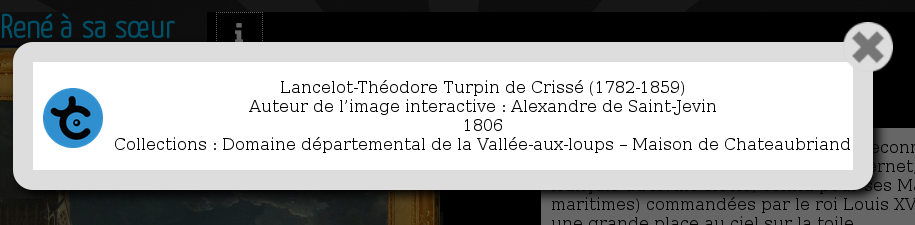
\includegraphics[width=\textwidth]{images/ia_title}\\
\end{center}

 The title entered in the metadata of the document appears above 
the interactive image and gives its name to the web page. The creator and 
 rights appear in the pop up associated with the "i" button 
on the right of the title of the interactive image.

You can save the image in svg format in the earlywork, 
through  \softmenu{File $\rightarrow$ Save as\ldots}.

For more clarity, you should remove the current extension of the image 
in the field \softmenu{Name} of the dialog window. Finally, in the 
dropdown menu, choose the Inkscape svg file format:

\softmenu{SVG Inkscape (*.svg)}.

Several Inkscape tools can be used to clip the details that
will become active in the animation generated by Xia. Among these:
\begin{itemize}
 \item 
\includegraphics[scale=0.5]{./images/square} \softmenu{Create rectangles and squares}
 \item 
\includegraphics[scale=0.5]{./images/circles} \softmenu{Create circles, ellipses and arcs}
 \item 
\includegraphics[scale=0.5]{./images/line} \softmenu{Draw freehand lines}
 \item 
\includegraphics[scale=0.5]{./images/bezier} \softmenu{Bezier curves and straight lines}
\end{itemize}

Without going in the detail of how these tools work\footnote{For this, 
refer to \href{http://inkscape.org/doc/shapes/tutorial-shapes.fr.html}{Inkscape manual} or \href{http://en.flossmanuals.net/inkscape/}{Floss manual}.} note that the tool "\softmenu{Draw Bezier curves and straight lines}" 
allows to crop "click by click" (work points are called 
"nodes").  You close the figure by clicking on the start node. 
You can draw "\softmenu{Bezier curves}" by keeping the mouse button pressed 
after creating a node, then moving the cursor to bring up the control handles 
to shape the curve segment as desired.


\begin{alert}
  If you set a left open shape in Inkscape (for example a line), Xia will automatically close it  by connecting a straight line between the beginning and the end of it.
\end{alert}

\begin{alert}
 The order of creation of details in Inkscape will be 
 the same in the html5 interactive image (for example: the first created detail in
Inkscape will appear at the top of the interactive image).
If you wish to change the sequence without having to create the details once more, see 
section \ref{XML_layer}.
\end{alert}

Once you have cut out a detail\footnote{The colour of the border will be the same in Inkscape and 
in the animation generated by Xia.}, you can select it with the tool  
\softmenu{Select and transform object} to resize it, move it\ldots

\begin{tip}
If you have some difficulties to select the details you have drawn,
apply a colour background to them. Choose whatever colour you like, except for black and white
(see why in section \ref{white_black_background}).
\end{tip}


You can access to the \softmenu{Object properties} by right-clicking on the cut-out detail.
Thus you also access to the dialog window in which you add the text to be associated with the 
detail in the interactive image:\\

\begin{center}
 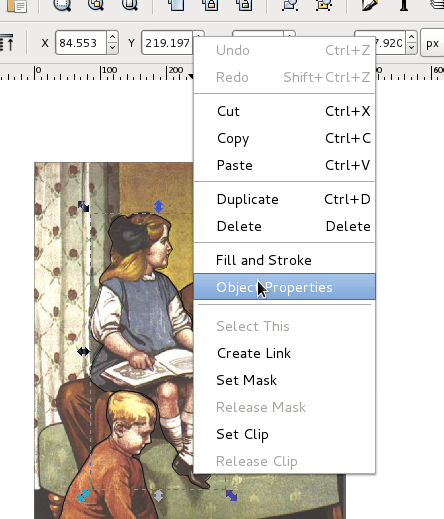
\includegraphics[width=0.5\textwidth]{./images/object_properties}\\ 
\end{center}

The two fields to be filled in this window are \softmenu{Title} and 
\softmenu{Description}.  The title filled in here will be that of the detail, 
description will be its comment. Do not forget to click on the \softmenu{Define}
button before you close the \softmenu {Object Properties} dialog window.

The process described above must also be done with the background image : 
the title and description indicated here will serve as an introduction to 
the interactive image (title and comment not related to a particular detail).

\subsection{Generating the interactive image with Xia}

When all the details are clipped and their metadata indicated, Xia can be launched (see figure \ref{xia_interface}).
You must select the svg source file with the top left icon\footnote{When launched as an Inkscape extension, the top
left icon has a different look, and can not be selected, since Xia assumes
you want to create the html5 animation from the image you are working on in Inkscape.},
choose the export options (see figure \ref{xia_export_options}), and then choose a 
template and the destination folder of the interactive image.


Clicking on one of the template icons generates a series of files and folders.
 Open the \softmenu{index.html} file in a 
  webbrowser to see the html5 interactive image.

\begin{alert}
This file will not display anything if used 
alone. All the other files and directories generated during the export process 
must be stored in  the same folder (see figure \ref{xia_files}) 
as the \texttt{index.html} file so that the animation works properly.
\textbf{It is therefore essential to 
dedicate a specific directory for each exported image}.
\end{alert}



\begin{figure}[htp]
\tikzstyle{box}=[draw, text width=4cm, fill=lightgray!50, rounded corners]
\begin{tikzpicture}
  %\draw[help lines] (0,0) grid (5,5);
  %icons
  \node (bBlue) {
\includegraphics[width=2cm]{./images/buttonBlue}};
  \node[left= .3mm of bBlue, opacity=.5] (aBrown) {
\includegraphics[width=2cm]{./images/audioBrown}};
  \node[right= .3mm of bBlue, opacity=.5] (guClic) {
\includegraphics[width=2cm]{./images/game1clic}};
  \node[below= .2mm of bBlue.south] (pBlue) {
\includegraphics[width=2cm]{./images/popBlue}};
  \node[left= .3mm of pBlue, opacity=.5] (gDDrop) {
\includegraphics[width=2cm]{./images/gameDragAndDrop}};
  \node[right= .3mm of pBlue] (pYellow) {
\includegraphics[width=2cm]{./images/popYellow}};
  \node[above = .2mm of guClic.north] (aCloud) {
\includegraphics[width=2cm]{./images/accordionCloud}};
  \node[above = .2mm of aCloud.north] (aBlack) {
\includegraphics[width=2cm]{./images/accordionBlack}};  
  \node[left = .3mm of aBlack] (params) {
\includegraphics[width=2cm]{./images/params}};  
  \node[left = .3mm of params] (files) {
\includegraphics[width=2cm]{./images/xia_open}};
  \node[left = 1mm of aCloud, opacity=.3] (xialogo) {
\includegraphics[height=2.1cm]{./images/xia}};
  
  %comments
  \node[box, text width=2.5cm,above left = 5mm of files] (filesC) {Select the svg source file};
  \node[box, above = 5mm of params] (paramsC) {Define the options of the export (see figure \ref{xia_export_options})};
  \node[box,above right = 5mm of aCloud.north east] (aBlackC) {\href{http://xia.dane.ac-versailles.fr/demo/tuto/xia1/accordionBlack}{accordionBlack}\\ Large comment zone, suitable for the insertion of multimedia resources; to be used with vertical images (portrait)};
  \node[box, right = 5mm of guClic] (aCloudC) {\href{http://xia.dane.ac-versailles.fr/demo/tuto/xia1/accordionCloud}{accordionCloud}\\ Narrow comment zone, with more space for the image itself ; to be used with horizontal images (landscape)};
  \node[box, below right = 5mm of pYellow] (pYellowC) {\href{http://xia.dane.ac-versailles.fr/demo/tuto/xia1/popYellow}{popYellow}\\ No lateral comment zone ; 
a first click on the detail reveals it, and a second one simultaneously unveils 
the comment and triggers the zoom function};
  \node[box, left = 25mm of bBlue] (bBlueC) {\href{http://xia.dane.ac-versailles.fr/demo/tuto/xia1/buttonBlue}{buttonBlue}\\ No lateral comment zone ; 
comments appear above the image (suitable for long comments) ; the users access  
the comments through icons placed above the interactive image};
  \node[box, below left = 5mm of pBlue] (pBlueC) {\href{http://xia.dane.ac-versailles.fr/demo/tuto/xia1/popBlue}{popBlue}\\ No lateral comment zone; 
a first click on the detail reveals it, and a second one pops up the comment 
(no zoom)};
  
  %arrows
  \draw[-stealth] (aBlackC.west) -- (aBlack.east);
  \draw[-stealth] (aCloudC.west) -- (aCloud.south east);
  \draw[-stealth] (pYellowC.north west) -- (pYellow.south east);
  \draw[-stealth] (bBlueC.north east) -- (bBlue.north west);
  \draw[-stealth] (pBlueC.north east) -- (pBlue.south west);
  \draw[-stealth] (filesC.south east) -- (files.north west);
  \draw[-stealth] (paramsC.south) -- (params.north);
  
\end{tikzpicture}
\caption{Xia's templates}
\label{xia_interface}
\end{figure}


\begin{figure}[htp]
\tikzstyle{box}=[draw, text width=4cm, fill=lightgray!50, rounded corners]
\begin{tikzpicture}
  %\draw[help lines] (0,0) grid (5,5);
  %icons
  \node (exp_qual) {
\includegraphics[scale=.5]{./images/exp_qual}};
  \node[right= .2mm of exp_qual] (exp_firefox) {
\includegraphics[scale=.5]{./images/exp_firefox}};
  \node[right= .2mm of exp_firefox] (exp_1file) {
\includegraphics[scale=.5]{./images/exp_1file}};
  
  %comments
  \node[box, text width=2.5cm, left = 5mm of exp_qual] (exp_qualC) {Select the quality of the export on a scale from 1 to 4};
  \node[box, above = 5mm of exp_firefox] (exp_firefoxC) {Activate or Deactivate the 
  creation of the FirefoxOS files (default: deactivated)};
  \node[box, text width=10cm, below = 5mm of exp_1file] (exp_1fileC) {In the unique file configuration,
  you will need an internet connection to access the resource. The xia engine
  used in the unique file configuration is hosted on Versailles academy servers
  and is automatically updated. In this configuration, you can not control the 
  background image and icons (default: deactivated)};

  %arrows
  \draw[-stealth] (exp_qualC.east) -- (exp_qual.west);
  \draw[-stealth] (exp_firefoxC.south) -- (exp_firefox.north);
  \draw[-stealth] (exp_1fileC.north) -- (exp_1file.south);

\end{tikzpicture}
\caption{Xia's exportation options}
\label{xia_export_options}
\end{figure}

\begin{figure}[htp]
\tikzstyle{every node}=[draw=black,thick,anchor=west]
\tikzstyle{auto}=[draw=reddebian,fill=reddebian!30, text height=2.5mm]
\tikzstyle{manual}=[draw=bluedane,fill=bluedane!30, text height=2.5mm]
\tikzstyle{manualT}=[fill=bluedane!30,draw=bluedane, rectangle,text width=5cm, rounded corners]
\tikzstyle{autoT}=[fill=reddebian!30,draw=reddebian, rectangle,text width=5cm, rounded corners]
\begin{tikzpicture}[%
  grow via three points={one child at (0.5,-0.7) and
  two children at (0.5,-0.7) and (0.5,-1.4)},
  edge from parent path={(\tikzparentnode.south) |- (\tikzchildnode.west)}]
  \node [manual] {my\_project/}
    child { node [auto] {index.html}}		
    child { node [auto] {deploy.html}}		
    child { node [auto] {manifest.webapp}}		
    child { node [auto] {css/}}
    child { node [auto] {data/}}
    child { node [auto] {font/}}
    child { node [auto] {img/}}
    child { node [auto] {js/}}
    child { node [manual] {videos/}
      child { node [manual] {video.mp4}}
      child { node [manual] {video.ogv}}
      child { node [manual] {video.webm}}
      };
  \node[manualT] (textM) at (10,-2) {These files and folders have been manually created by the interactive image designer. The folder \textcolor{bluedane}
{videos} was also manually created, in order to host videos inserted 
in the comments of the interactive image using relative links.}; 
  \node[autoT] (textA) at (10,-6) {Files and folders generated by Xia from the svg source file.};
  \draw[-stealth] (textM.west) -- (4,0);
  \draw[-stealth] (textM.west) -- (5.5,-7);
  \draw[-stealth] (textA.west) -- (4,-3);
\end{tikzpicture}
\caption{Files of an interactive image with FirefoxOS export activated}
\label{xia_files}
\end{figure}

In fact, since Xia is also an Inkscape plugin, you can generate your project directly 
in Inkscape: just click on \softmenu{Plugins $\rightarrow$ Various $\rightarrow$ Xia Édu}, 
and choose your template and destination folder.

\begin{tip}
 If you use GNU/Linux or Mac OS X, you can generate your html5 animation
 using the terminal with the command \texttt{xia-converter}. The parameters are
 \texttt{-i} to indicate the input file, \texttt{-o} to indicate the exportation folder, and
 \texttt{-t} to indicate the template.\\
 \emph{GNU/Linux}\\
 \texttt{\$ xia-converter -i myfile.svg -o export\_folder/ -t accordionBlack}\\
 \emph{Mac OS X}\\
 \texttt{\$ cd /Applications/xia.app/Contents/Resources/}\\
 \texttt{\$ python xia.py -i myfile.svg -o export\_folder/ -t gameDragAndDrop}\\
 The template accordionBlack will be chosen if a syntax error is made in the \texttt{-t} parameter.
\end{tip}


\subsection{Abstract}

\begin{enumerate}
 \item An interactive image is first built in Inkscape (svg format). Xia only 
 converts the svg source file into an html5 animation ;
 \item The title of the interactive image must be indicated in the \softmenu{Metadata of 
the document} ;
 \item The text of the details must be filled in the \softmenu{Object properties}, 
 in the \softmenu{Title} and \softmenu{Description} fields of the cut out details ;
 \item The general description of the interactive image must be indicated in the \softmenu
{Object properties} of the background image.
\end{enumerate}

\section{Enriched interactive image}\label{enriched_IA}

\begin{links}
Explore the \href{http://xia.dane.ac-versailles.fr/demo/tuto/xia2}{interactive image} created for this section of the documentation.

Download the \href{http://xia.dane.ac-versailles.fr/demo/tuto/xia2/svg/xia2.svg}{svg} source file.
\end{links}

In this section, the goal is still to create a "traditional" interactive image 
(ie. in which a detail matches with a comment), but the content of the comments 
will be enriched with  formatted text or multimedia resources.


\newpage
\subsection{Formatting text}

In order to insert formatted text, the tags described in figure \ref{xia_text_tags} should be used.

\begin{figure}[htp!]
\tikzstyle{descrip}=[font=\sffamily, anchor=north west, text width = 4.3cm]
\tikzstyle{box}=[draw, text width=4cm, fill=lightgray!50, rounded corners, anchor=north west]
\begin{tikzpicture}
  \node[anchor=north west] (bold) {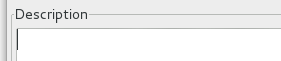
\includegraphics[scale=.5]{./images/Description}};
  \node[descrip, below = -7mm of bold] (boldT) {This text is ***bold***};
  \node[box, right = 3.5cm of bold] (bolR) {This text is in \textbf{bold}};
  \node[anchor=north west, below = .2cm of bold] (italic) {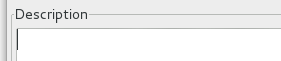
\includegraphics[scale=.5]{./images/Description}};
  \node[descrip, below = -7mm of italic] (italicT) {This text is in **italics**};
  \node[box, right = 3.5cm of italic] (italicR) {This text is in \textit{italics}};
  \node[anchor=north west, below = .2cm of italic] (texttt) {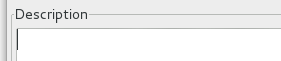
\includegraphics[scale=.5]{./images/Description}};
  \node[descrip, below = -7mm of texttt] (textttT) {This text is in \verb!{{{typewriter}}}!};
  \node[box, right = 3.5cm of texttt] (textttR) {This text is in \texttt{typewriter}};
  \node[anchor=north west, below = .2cm of texttt] (link) {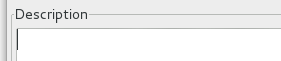
\includegraphics[scale=.5]{./images/Description}};
  \node[descrip, below = 7mm of link.north] (linkT) {A link to \verb![https://www.wikipedia.org/ Wikipedia]!};
  \node[box, right = 3.5cm of link] (linkR) {A link to \href{https://www.wikipedia.org/}{Wikipedia}}; 
  \node[anchor=north west, below = .2cm of link] (relativelinks) {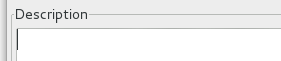
\includegraphics[scale=.5]{./images/Description}};
  \node[descrip, below = -7mm of relativelinks] (relativelinksT) {A link to a \verb![/home/foo/bar.pdf local file]!};
  \node[box, right = 3.5cm of relativelinks] (relativelinksR) {A link to a \href{/home/foo/bar.pdf}{local file\footnote{That does not work on your computer!}}};
  \node[anchor=north west, below = .8cm of relativelinks] (bullets) {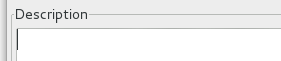
\includegraphics[scale=.5]{./images/Description}};
  \node[descrip, below = -7mm of bullets] (bulletsT) {Making a list \\ $\ast$ of bullets \\  $\ast$ out of \\ ~$\ast$ 2 levels\footnote{Insert a \Spacebar (space) before the $\ast$}};
  \node[box, right = 3.5cm of bullets.south east] (bulletsR) {Making a list 
      \begin{itemize}
       \item of bullets
       \item out of
       \begin{itemize}
         \item2 levels
       \end{itemize}
      \end{itemize}};
  \node[anchor=north west, below = 3cm of bullets] (line) {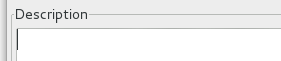
\includegraphics[scale=.5]{./images/Description}};
  \node[descrip, below = 7mm of line.north] (lineT) {Drawing \\ - - - - \\ a line};
  \node[box, right = 3.5cm of line] (lineR) {Drawing \\ \hrulefill \\ a line};
\end{tikzpicture}
\caption{Tags to format text}
\label{xia_text_tags}
\end{figure}

\subsection{Inserting multimedia resources into details}\label{multimedia_enrichment}

Inserting multimedia resources into details comments is quite easy: just paste 
the resource url (relative or absolute link) or iframe tag of the web service 
you want to use. Xia will automatically create a multimedia player in the comment as long as 
the resource (image, sound or video) matches its supported formats: 
\begin{description}
 \item [Images] jpg, jpeg, png, gif
 \item [Audio] ogg, mp3
 \item [Video] ogv, webm, mp4
\end{description}

The link has to be inserted into the \softmenu{Description} field of the \softmenu{Object Properties}.

\begin{description}
 \item[Absolute link] If the resource url is
 
 %\begin{center}
 \verb|http://web.crdp.ac-versailles.fr/02546.ogg|
 %\end{center}
 
 just type it in the \softmenu{Description} field of the \softmenu{Object Properties} in 
 Inkscape
 
 \item [Relative link] If the multimedia file is located in the interactive image 
 folder or in a folder (see figure \ref{xia_files}) within this one, just indicate its location, keeping in 
 mind that the interactive image folder has to be considered as the root folder. 
 For example, if the \verb|video.ogv| file is located in a \verb|videos| 
 folder located itself in the interactive image exportation folder, just indicate:
 
 %\begin{center}
  \verb|./videos/video.ogv|
 %end{center}
 
  in order to create the player. The \verb|./| means that the \verb|videos| folder
  is located in the exportation folder. You can also use the \verb|../| tag to indicate
  that the resource is located in a parent folder.
\end{description}

\begin{tip}
Since video formats supported by Xia are not natively supported by every web 
browsers, it is recommanded to export videos into the 3 supported formats, 
and to upload them into a single folder (from there, the only difference 
between these files is their extension, ie. .ogv or .mp4 or .webm).
Even if a particular format is indicated in the description (following 
the previous example : \verb|videos/video.ogv|), if the browser is 
unable to read the resource, it will automatically attempt to read the files 
of the same name possessing a different extension (ie. \verb|video.mp4| 
then \verb|video.webm|).
\end{tip}

The last option is to insert an iframe tag.
It will be interpreted and the reader will appear in the comment, 
giving access to the resource.

\subsection{The "audioBrown" template: sounds instead of text}\label{audioBrownsection}

\begin{links}
Explore the \href{http://xia.dane.ac-versailles.fr/demo/tuto/xia4}{interactive image} created for this section of the documentation.

Download the \href{http://xia.dane.ac-versailles.fr/demo/tuto/xia4/svg/xia4.zip}{svg} source file (zip file containing the svg source file
and the sounds).
\end{links}

The "audioBrown" template is specifically dedicated to the creation of 
interactive images in which details are associated with sounds instead of text.

The method to insert sounds using absolute or relative links is described in 
section 
\ref{multimedia_enrichment}. If you wish the sound to play 
automatically as the user clicks on the comment, just add \verb|autostart| right 
after the url \footnote{The "\texttt{autostart}" tag also works with the other 
Xia templates.}:\\
\begin{center}
 \verb|sounds/detail_1_sound.ogg autostart|
\end{center}


\subsection{Inserting images into your interactive image}\label{insertion_images}

Png images can be added to the background. To do so, select \softmenu{File $\rightarrow$ Import} in 
Inkscape to incorporate your new image.

The imported image will only appear in the html5 animation if you have applied white background in 
Inkscape. Choose white in the horizontal colour palette at the bottom of 
Inkscape interface:\\

\begin{center}
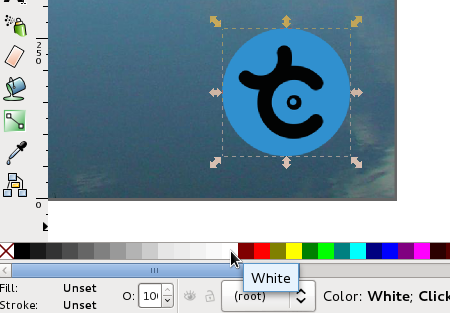
\includegraphics[width=0.6\textwidth]{images/white_fill}\\ 
\end{center}


By indicating a url in the \softmenu{Title} of \softmenu{Object properties} field, 
the embedded image becomes a clickable icon linking to a web page.

\subsection{Displaying a question and unveiling an answer}

You can create clickable icon which will momentarily 
prevent the user to read the end of the comment.
You can even ask the user to enter a password to read the 
end of the comment.

To do so, just indicate, in the description, the tags described in figure \ref{xia_answer_tags}.

\begin{figure}[htp!]
\tikzstyle{descrip}=[font=\sffamily, anchor=north west, text width = 4.3cm]
\tikzstyle{box}=[draw, text width=6cm, fill=lightgray!50, rounded corners, anchor=north west]
\begin{tikzpicture}
  \node[anchor=north west] (answer) {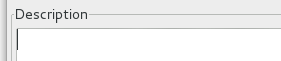
\includegraphics[scale=.5]{./images/Description}};
  \node[descrip, below = -7mm of answer] (answerT) {[[Can I ask you a question? (code=12345): Yes, indeed I can.]]};
  \node[box, right = 3.5cm of answer] (answerI) {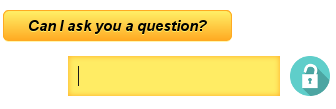
\includegraphics[scale=.5]{./images/answer_code}};
\end{tikzpicture}
\caption{Tags to insert a button which will momentarily prevent the user to read the end of the comment}
\label{xia_answer_tags}
\end{figure}

Use the double brackets tag \texttt{[[ (...) ]]} to indicate you wish to create the icon, 
split the text between the question and the answer with the \texttt{:}
tag, and add a code by inserting \texttt{(code=insert\_password)} just before 
the \texttt{:} tag\footnote{The \texttt{(code={...})} is not mandatory. Remember 
that you can not insert the \texttt{)} character in the password.}.
  
\subsection{Controlling details behavior : automatic display and disabled zoom}\label{white_black_background}

Default behavior of details in an interactive image consists in:
\begin{itemize}
 \item highlighting details only on mouse over or with a click on the comment 
 detail title
 \item zoom in effect when clicking again on the active detail\footnote{Except 
 for the popBlue template.}
\end{itemize}

Both of these default behaviors can be modified if you apply a white
 or black background to cropped details (see section 
\ref{insertion_images}):
\begin{description}
 \item [Detail with a white background] In the generated image, details will be
 immediately visible as a flat area of opaque color, hiding the background image;  
 once selected, it reveals the background (the zoom effect is still active).
 \item [Detail with a black background] Users still have to click on the detail to unveil it, but the zoom effect is disabled.
\end{description}

Logical consequence : you can not apply a white and a black background all together on the same detail.
A single detail can not be immediately displayed and have the zoom effect disabled.

\subsection{Controlling order of details display in the lateral comment zone}\label{XML_layer}

By default, in the interactive image, the details appear vertically following the order
in which these details have been created (the first detail created in Inkscape corresponding 
to the detail placed up in the sidebar of the interactive image).

We will work with the \softmenu{Edit $\rightarrow$ XML Editor} to change this default order.

A priori complex to manage, this dialogue window is in fact quite easy to use : 
by selecting the input in the XML editor, the corresponding detail will be
highlighted on the image and the only thing left 
to do is to drag the files to the desired location:\\

\begin{center}
 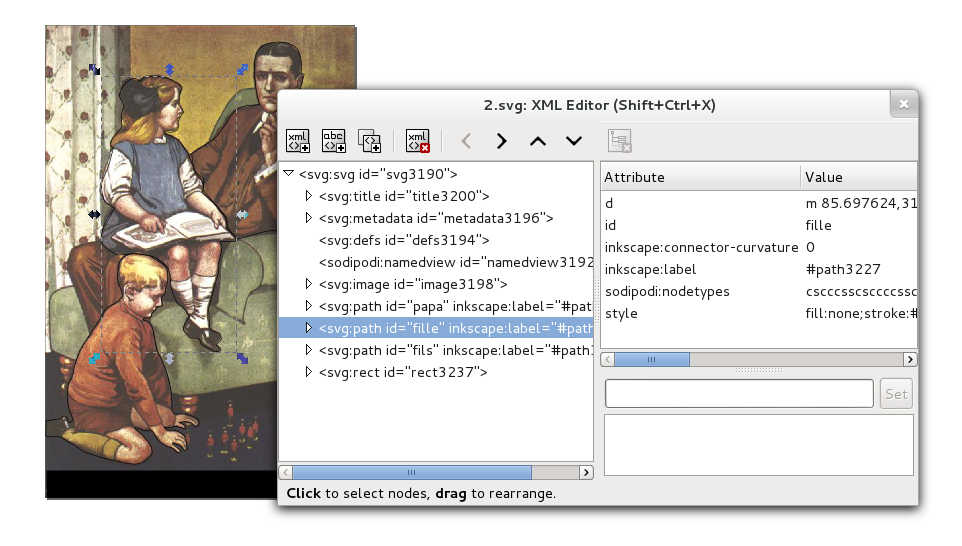
\includegraphics[width=\textwidth]{images/layerorder}\\
\end{center}
 
 The Inkscape XML editor allows to control the display order of the details 
in the interactive image. Note the highlighting of an element  
in the editor and on the background image by a single mouse click.

\subsection{Abstract}

\begin{enumerate}
 \item You can enrich and shaping text using tags
 \item A multimedia enrichment is possible through a simple link (relative
or absolute) to a file whose format is recognized by Xia
 \item Adding images to the background image is possible by importing them and applying them a white background
 \item It is possible to modify the default behavior of a detail by changing its color 
background (white, black)
 \item The order of the details in the interactive image depends on the order
of their creation in Inkscape. Nevertheless, the Inkscape XML editor allows to change this order
\item It is possible prevent the user to access the comments by inserting a clickable icon and / or a password
\end{enumerate}

\newpage

\section{Creating games with Xia}\label{games_IA}

Until now, this document was only about creation of traditionnal "interactive images": 
background image enriched with cropped details associated with texts.

This kind of interactive image can be used in class in various situations 
(students progressively discovering a document, or creating an interactive image
on their own), but Xia introduces new features, 
such as the creation of games and activities, in which the final user 
has much more to do than simply clicking on details in order to read the comment.

\begin{figure}[htp]
\tikzstyle{box}=[draw, text width=4cm, fill=lightgray!50, rounded corners]
\begin{tikzpicture}
  %\draw[help lines] (0,0) grid (5,5);
  %icons
  \node[opacity=.5] (bBlue) {
\includegraphics[width=2cm]{./images/buttonBlue}};
  \node[left= .3mm of bBlue] (aBrown) {
\includegraphics[width=2cm]{./images/audioBrown}};
  \node[right= .3mm of bBlue] (guClic) {
\includegraphics[width=2cm]{./images/game1clic}};
  \node[below= .2mm of bBlue.south, opacity=.5] (pBlue) {
\includegraphics[width=2cm]{./images/popBlue}};
  \node[left= .3mm of pBlue] (gDDrop) {
\includegraphics[width=2cm]{./images/gameDragAndDrop}};
  \node[right= .3mm of pBlue, opacity=.5] (pYellow) {
\includegraphics[width=2cm]{./images/popYellow}};
  \node[above = .2mm of guClic.north, opacity=.5] (aCloud) {
\includegraphics[width=2cm]{./images/accordionCloud}};
  \node[above = .2mm of aCloud.north, opacity=.5] (aBlack) {
\includegraphics[width=2cm]{./images/accordionBlack}};  
  \node[left = .3mm of aBlack] (params) {
\includegraphics[width=2cm]{./images/params}};  
  \node[left = .3mm of params] (files) {
\includegraphics[width=2cm]{./images/xia_open}};
    \node[left = 2mm of aCloud, opacity=.3] (xialogo) {
\includegraphics[height=2cm]{./images/xia}};

  
  %comments
  \node[box, text width=2.5cm,above left = 5mm of files] (filesC) {Select the svg source file};
  \node[box, above = 5mm of params] (paramsC) {Define the options of the export (see figure \ref{xia_export_options})};
  \node[box, right = 5mm of guClic] (guClicC) {\href{http://xia.dane.ac-versailles.fr/demo/tuto/xia3}{game1clic}\\ 
  selecting details on a background image \\ How-to in section \ref{game1clicsection}};
  \node[box, left = 25mm of bBlue] (aBrownC) {\href{http://xia.dane.ac-versailles.fr/demo/tuto/xia4}{audioBrown} \\ creation of interactive images in
  which details are associated with sounds \\ How-to in section \ref{audioBrownsection}};
  \node[box, below left = 5mm of pBlue] (gDDropC) {\href{http://xia.dane.ac-versailles.fr/demo/tuto/xia5}{gameDragAndDrop}\\ 
  drag and drop graphical elements on the background images \\ How-to in section \ref{gameDragAndDropsection}};
  
  %arrows
  \draw[-stealth] (guClicC.west) -- (guClic.east);
  \draw[-stealth] (gDDropC.north) -- (gDDrop.south west);
  \draw[-stealth] (aBrownC.east) -- (aBrown.west);
  \draw[-stealth] (filesC.south east) -- (files.north west);
  \draw[-stealth] (paramsC.south) -- (params.north);
  
\end{tikzpicture}
\caption{Xia's games and multimedia templates}
\label{xia_interface2}
\end{figure}

\subsection{First game principle: selecting, finding elements in the image}\label{game1clicsection}

% \begin{wrapfigure}{r}{45mm}
%   \centering
%   
\includegraphics[scale=0.7]{./images/game1clic} 
% \end{wrapfigure}

\textit{The game principle described in this section consists in selecting details 
on a background image. When the user has reached the goal described in the 
instructions, a message appears in a final pop up.}


\begin{links}
Explore the \href{http://xia.dane.ac-versailles.fr/demo/tuto/xia3}{interactive image}
created for this section of the documentation.

Download the \href{http://xia.dane.ac-versailles.fr/demo/tuto/xia3/svg/xia3.svg}{svg} source file.
\end{links}

This kind of game is almost the easiest way to create an interactive image.
You only have to crop the details that the final user will have to select. 

The instructions must be completed in the 
metadata of the document. Xia will look into 
the informations  filled in the \softmenu{Description} field of the metadata of the document
(see section \ref{preparation_svg}: \softmenu{File $\rightarrow$ Metadata of the document}), 
and create an instruction «~pop up~» that will show up at the opening of the game. The player 
will just have to read the instructions and close the pop up to play the game.

When the user completes the game, a message automatically appears.
This message has to be filled in the \softmenu{Description} field of the \softmenu{Object Properties} of the 
background image. 

Two informations are needed in order for this message to pop up :
the exact number of details that have to be selected\footnote{This number does 
not have to match the number of details on the image.}
and the message itself (see table \ref{tag1_sumup}).

\begin{table}
 \begin{tabular}{|l|p{2in}|p{2in}|}
 \hline
  Goal & Enter the number of correct answers needed to complete the game & Display a message\\
  \hline
  Tag & \texttt{<score></score>}| & \texttt{<message></message>}\\
  \hline
  Example & \multicolumn{2}{|l|}{\texttt{<score>6</score>}}\\
   & \multicolumn{2}{|l|}{\texttt{<message>Congratulations!}}\\
    & \multicolumn{2}{|l|}{\texttt{You have completed the game!</message>}}\\
  \hline
 \end{tabular}
\caption{Sum up of tags in a game1clic game}
\label{tag1_sumup}
\end{table}
 
\begin{tip}
Text inserted inside the \verb|<message></message>| tag can be 
enriched. Images, videos or sounds can be inserted.
It is also possible to insert a link, allowing users to play another game,
in order to "chain" activities up by degree of difficulty.
\end{tip}


Once your svg source file is created, choose the template \softmenu{game1clic} to generate the interactive game.

\subsection{Second game principle: classyfying, ordering, ranking}\label{gameDragAndDropsection}

% \begin{wrapfigure}{r}{45mm}
%   \centering
%   
\includegraphics[scale=0.7]{./images/gameDragAndDrop} 
% \end{wrapfigure}

\textit{The second kind of game that can be created with Xia consists in
dragging and dropping graphical elements on the background image. If all the
elements have been dropped on their corresponding drop zone, a pop up
message appears, confirming the achievement of the game.}

\begin{links}
Explore the \href{http://xia.dane.ac-versailles.fr/demo/tuto/xia5}{interactive image}
created for this section of the documentation.

Download the \href
{http://xia.dane.ac-versailles.fr/demo/tuto/xia5/svg/xia5.svg}{svg} source file.
\end{links}

This is how you can create a game based on the drag and drop principle :
\begin{enumerate}
 \item In Inkscape:
\begin{itemize}
 \item Choose and import a background picture
 \item Create the graphical elements the users of the interactive image will have to drag and drop (ie. images or group of words: see below for a how-to)
 \item Create the instruction pop up in \softmenu{File $\rightarrow$ Metadata of the document $\rightarrow$ Description}\footnote{Exactly as in the game1clic template.}
 \item Using metadata, make each label match its drop zone (actually being cropped details)
\end{itemize}
 \item In Xia
 \begin{itemize}
  \item Export the svg source file using the \softmenu{gameDragAndDrop} template
 \end{itemize}
\end{enumerate}

Two methods can be used to create the drag and drop "graphical-elements".
A very simple way is to use a screenshot tool, in order to create png files, and then import them in Inkscape.
It is also possible to create these elements directly in Inkscape, by creating a text, grouping it with a shape,
and finally making a bitmap copy of this group (\softmenu{Edition $\rightarrow$ Make a bitmap copy})


The graphical elements then have to be associated with their drop zone \footnote{\textbf{One} object
can only match \textbf{one} drop zone.}. In order to do that, make the \softmenu{ID} field of the drop zone match
the \softmenu{Description} field of the drag and drop graphical element. 
The only subtlety consists in the  \verb|<target></target>| tags which have to be filled in the \softmenu
{Description} field.

You will find in the table \ref{tag2_sumup} an abstract of the metadata to be filled in the \softmenu{Object Properties} 
of the drag and drop graphical elements and the corresponding details in order to make them match.

\begin{table}
\begin{tabular}{|p{1.in}|p{2.5in}|p{1.5in}|}
\hline
 & Graphical element (drag and drop objects in the game) & Cropped detail (drop zone)\\
\hline
ID Field & & \verb|Detail_Title|\\
\hline
Description Field & \verb|<target>Detail_Title</target>| & \\
\hline
\end{tabular}
\caption{Sum up of tags in the gameDragAndDrop template}
\label{tag2_sumup}
\end{table}

Once your svg source file is created, choose the template \softmenu{gameDragAndDrop} to generate the interactive game.

\subsection{Third game principle: collisions}

\textit{The game principle described in this section consists in moving objects
within bounds you defined. Typically, the "collisions" game principle
can be used to create mazes or gem puzzle.}

\begin{links}
Explore the \href{http://xia.dane.ac-versailles.fr/demo/tuto/xia6/}{interactive image}
created for this section of the documentation.

Download the \href
{http://xia.dane.ac-versailles.fr/demo/tuto/xia6/svg/xia6.svg}{svg} source file.
\end{links}

In order to create this kind of game, add the tag \verb|<collisions>on</collisions>| to the 
background image. All the details will then become solid and will prevent objects 
(png imported files or bitmap copies of shapes created in Inkscape) from being moved through them.

The "collision" game is in fact a gameDragAndDrop game, since the goal remains to 
drag one or several objects and drop them somewhere on the image.
The requisite tags for this template are therefore the same as in the gameDragAndDrop
template \footnote{\texttt{<target></target>} on the objects, \texttt{<score></score>} 
and \texttt{<message></message>} on the background image: see section \ref{gameDragAndDropsection}.}, but you 
will apply the \verb|<collisions>off</collisions>| tag to the drop zone's \softmenu{Description} field.

Once your svg source file is created, choose the template \softmenu{gameDragAndDrop} to generate the interactive game.

\subsection{\emph{Advanced interactive games creation tips}: Magnet effect, tooltips, double-scoring\ldots}

\subsubsection{Showing the player's score (game1clic template)}\label{playersscore}

It is possible to display graphical elements automatically  when the user 
selects the correct answer. These elements can be png imported images or shapes directly designed in
Inkscape.
But as Xia considers as a clickable 
detail any shapes designed using Inkscape tools, you 
will have to transform these shapes in bitmap, using the "bitmap copy" Inkscape tool. 
For example :
\begin{enumerate}
 \item Draw  a star with yellow sides on a yellow background with the Inkscape tools 
 \item Select this star, and click on the \softmenu{Edition $\rightarrow$ Make a bitmap copy}
 \item Delete the first star
\end{enumerate}

When the graphical elements are imported (png files) or created (bitmap copy 
of shapes created manually), just apply the following 
carasteristics to these elements:
\begin{center}
\softmenu{Interactivity > OnClick} = \verb|off|
\end{center}
Then, group the clickable detail to its graphical element (by successively 
clicking on the detail and the graphical element with the \Shift keystroke on),
then select \softmenu{Group} in the Inkscape \softmenu{Object} menu.

\subsubsection{Showing the player's mistakes (game1clic template)}

Games based on the details selection principle are obviously very
interesting educational games\ldots but it is also quite obvious to guess how some 
students may be tempted to cheat to achieve such games (for example, by 
frenetically clicking everywhere on the image, until the final message pops up).

This is why it may be interesting to be able to 
highlight the user's mistakes during the game.

To do so, you will anticipate the user's probable mistakes, and 
put explicit graphical elements symbolizing these errors on the background image. 
This graphical element may be an imported image 
(png file) or a shape directly designed with the Inkscape tools, 
then converted into bitmap (see section \ref{playersscore}).. These elements will have to include the following caracteristics:
\begin{center}
\softmenu{Interactivity > OnClick} = \verb|disable-score| 
\end{center}
When applied with a \verb|disable-score| tag, a detail still remains clickable, but does not 
add a score to the counter that delivers the final success message pop up.


\subsubsection{How to add a "magnet" effect (gameDragAndDrop template)}

If you indicate \verb|<magnet>on</magnet>| in the \softmenu{Description} field of the drop zone, a magnet effect will then be active when the player drops the 
graphical element onto its matching drop zone.

\subsubsection{Links on drop zones (gameDragAndDrop template)}
 
You can insert links in the \softmenu{Title} field of the \softmenu{Object Properties} 
of the drop zones. The user can then open the link by clicking on it or by dropping its 
corresponding detail on it.


\subsubsection{Tooltips (game1clic and gameDragAndDrop templates)}

\begin{links}
Explore the \href{http://xia.dane.ac-versailles.fr/demo/tuto/xia7}{interactive image}
created for this section of the documentation.

Download the \href{http://xia.dane.ac-versailles.fr/demo/tuto/xia7/svg/xia7.svg}{svg} source file.
\end{links}

It is possible to display tooltips of details on mouse-over. To do so, 
create the tooltip with a png imported file or a bitmap copy (see section \ref{playersscore})
of a text created in 
Inkscape\footnote{Or a bitmap copy of a shape grouped with some text\ldots}, and 
apply to this tooltip a specific \softmenu{ID} in its \softmenu{Object Properties}. Then, 
just apply the tag \verb|<tooltip>specific_ID_of_the_tooltip</tooltip>| in the 
\softmenu{Description} field of the \softmenu{Object Properties} of the detail that is supposed 
to make the tooltip appear (for example, in the image below: on mouse-over, the
yellow square makes the tooltip ``Test'' appear):\\


\begin{center}
 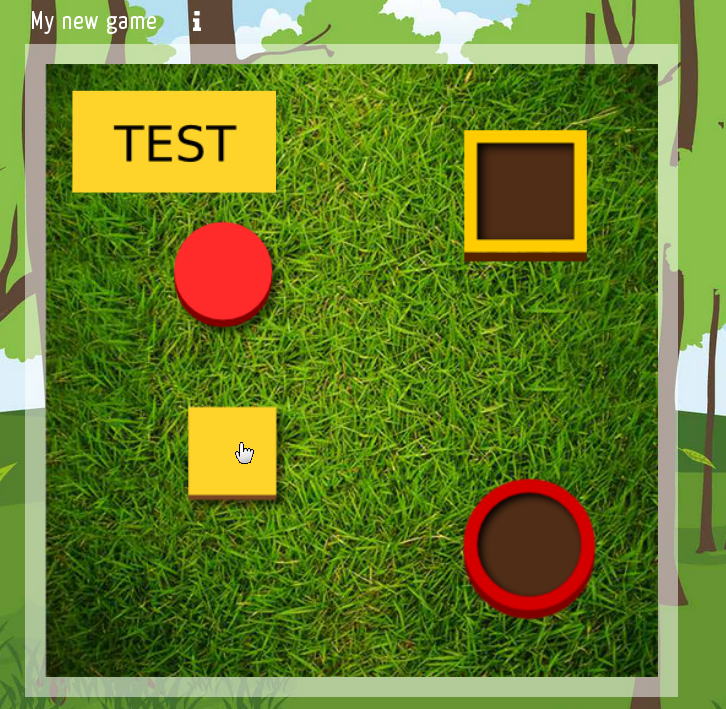
\includegraphics[width=0.5\textwidth]{images/tooltip_example}\\
 \end{center}

Note that the tooltip tool is available in the game1clic and in the gameDragAndDrop templates.\\
 

\subsubsection{Double scoring (game1clic and gameDragAndDrop templates)}

If you indicate \verb|score2| in the \softmenu{onclick} field
(\softmenu{Object Properties $\rightarrow$ Interactivity}) of the detail,
and if you use \texttt{<score2></score2>} and  \texttt{<message2></message2>} 
in the \softmenu{Object Properties} of the 
background image, you create a double scoring game. In this kind of game, the
user can select two different categories of details, 
two messages can pop up at the end, depending on the category and number
of details the user has selected.

For example, you can create a game with 3 details tagged with \texttt{score2}
(corresponding to mistakes), and indicate in the \softmenu{Object Properties}
of the background image:\\
\texttt{<score>4</score>\\
<message>Hurray!</message>\\
<score2>3</score2>\\
<message2>Three mistakes... that is a bit too much... Concentrate more and do it again</message2>}\\

\newpage
\subsection{Abstract}

These tables sum up the tags that have to be indicated when a game is created:

\begin{table}[thp]
 \begin{tabular}{|p{.5cm}|p{2cm}|p{10cm}|}
 \hline
 \multicolumn{3}{|l|}{\softmenu{game1clic} template} \\
 \hline
 \multicolumn{3}{|l|}{\texttt{<score></score>}}\\
 \hline
 & \emph{Role} & Sets the amount of correct answers needed to pop up the end message of the game\\
 & \emph{Element}  & Background picture \\
 & \emph{Where ?} & \softmenu{Object properties $\rightarrow$ Description} \\
 & \emph{What ?} & A number corresponding to the required score\\
 \hline
 \multicolumn{3}{|l|}{\texttt{<message></message>}}\\
 \hline
  & \emph{Role} & Pops up the end message of the game \\
  & \emph{Element}  & Background picture \\
  & \emph{Where ?} & \softmenu{Object properties $\rightarrow$ Description}\\ 
  & \emph{What ?} & A personalized message if necessary enriched with multimedia or html links\\
  \hline
  \multicolumn{3}{|l|}{\texttt{off}}\\
  \hline
  & \emph{Role} & Makes a cropped detail unclickable \\
  & \emph{Element} & Detail \\
  & \emph{Where ?} & \softmenu{Object properties $\rightarrow$ Interactivity $\rightarrow$ Onclick}\\
 \hline
  \multicolumn{3}{|l|}{\texttt{disable-score}}\\
  \hline
  & \emph{Role} & Makes a cropped detail clickable, but when clicked, does not add a point to the score game counter \\
  & \emph{Element} & Detail \\
  & \emph{Where ?} & \softmenu{Object properties $\rightarrow$ Interactivity $\rightarrow$ Onclick}\\
  \hline
    \multicolumn{3}{|l|}{\texttt{score2}}\\
  \hline
  & \emph{Role} & Makes a detail add a score to the score2 counter \\
  & \emph{Element} & Detail \\
  & \emph{Where ?} & \softmenu{Object properties $\rightarrow$ Interactivity $\rightarrow$ Onclick}\\
  \hline
  \multicolumn{3}{|l|}{\texttt{<tooltip></tooltip>}}\\
  \hline
  & \emph{Role} & Displays a tooltip when moused-over \\
  & \emph{Element} & Detail \\
  & \emph{What ?} & Make sure to match the ID of the element used as tooltip\\
  & \emph{Where ?} & \softmenu{Object properties $\rightarrow$ Description}\\
  \hline
 \multicolumn{3}{|l|}{\texttt{<score2></score2>}}\\
 \hline
 & \emph{Role} & Sets the amount of correct answers needed to pop up the second end message in a double scoring game\\
 & \emph{Element}  & Background picture \\
 & \emph{Where ?} & \softmenu{Object properties $\rightarrow$ Description} \\
 & \emph{What ?} & A number corresponding to the required score\\
 \hline
 \multicolumn{3}{|l|}{\texttt{<message2></message2>}}\\
 \hline
  & \emph{Role} & Pops up the second end message in a double scoring game \\
  & \emph{Element}  & Background picture \\
  & \emph{Where ?} & \softmenu{Object properties $\rightarrow$ Description}\\ 
  & \emph{What ?} & A personalized message if necessary enriched with multimedia or html links\\
  \hline
  \end{tabular}
  \caption{Complete game1clic tags}
 \end{table}
 
 \begin{table}[thp]
 \begin{tabular}{|p{.5cm}|p{2cm}|p{10cm}|}
 \hline
 \multicolumn{3}{|l|}{\softmenu{gameDragAndDrop} template} \\
 \hline
 \multicolumn{3}{|l|}{\texttt{<score></score>}}\\
 \hline
 & \emph{Role} & Sets the amount of correct answers needed to pop up the end message of the game\\
 & \emph{Element}  & Background picture \\
 & \emph{Where ?} & \softmenu{Object properties $\rightarrow$ Description} \\
 & \emph{What ?} & A number corresponding to the required score\\
 \hline
 \multicolumn{3}{|l|}{\texttt{<message></message>} }\\
 \hline
  & \emph{Role} & Pops up the end message of the game \\
  & \emph{Element}  & Background picture \\
  & \emph{Where ?} & \softmenu{Object properties $\rightarrow$ Description}\\ 
  & \emph{What ?} & A personalized message if necessary enriched with multimedia or html links\\
  \hline
  \multicolumn{3}{|l|}{\texttt{<target></target>}}\\
  \hline
  & \emph{Role} & Indicates the corresponding drag and drop element and drop zone \\
  & \emph{Element} & Graphical element to move \\
  & \emph{Where ?} & \softmenu{Object Properties $\rightarrow$ Description}\\
  & \emph{What ?} & Make sure to match the ID field of the drop zone\\
  \hline
  \multicolumn{3}{|l|}{\texttt{<magnet>on</magnet>}}\\
  \hline
  & \emph{Role} & Adds a "magnet" effect \\
  & \emph{Element} & Drop zone \\
  & \emph{Where ?} & \softmenu{Object Properties $\rightarrow$ Description} \\
  \hline
  \multicolumn{3}{|l|}{\texttt{<collisions>on</collisions>}}\\
  \hline
  & \emph{Role} & Activates the "collisions" game principle \\
  & \emph{Element} & Background picture \\
  & \emph{Where ?} & \softmenu{Object Properties $\rightarrow$ Description} \\
  \hline
  \multicolumn{3}{|l|}{\texttt{<collisions>off</collisions>}}\\
  \hline
  & \emph{Role} & Creates a drop zone in a "collisions" game\\
  & \emph{Element} & Drop zone\\
  & \emph{Where ?} & \softmenu{Object Properties $\rightarrow$ Description} \\
  \hline
    \multicolumn{3}{|l|}{\texttt{<tooltip></tooltip>}}\\
  \hline
  & \emph{Role} & Displays a tooltip when moused-over \\
  & \emph{Element} & Drop zone, Graphical element to move \\
  & \emph{What ?} & Make sure to match the ID of the element used as tooltip\\
  & \emph{Where ?} & \softmenu{Object properties $\rightarrow$ Description}\\
  \hline
 \multicolumn{3}{|l|}{\texttt{<score2></score2>}}\\
 \hline
 & \emph{Role} & Sets the amount of correct answers needed to pop up the second end message in a double scoring game\\
 & \emph{Element}  & Background picture \\
 & \emph{Where ?} & \softmenu{Object properties $\rightarrow$ Description} \\
 & \emph{What ?} & A number corresponding to the required score\\
 \hline
 \multicolumn{3}{|l|}{\texttt{<message2></message2>}}\\
 \hline
  & \emph{Role} & Pops up the second end message in a double scoring game \\
  & \emph{Element}  & Background picture \\
  & \emph{Where ?} & \softmenu{Object properties $\rightarrow$ Description}\\ 
  & \emph{What ?} & A personalized message if necessary enriched with multimedia or html links\\
  \hline
  \end{tabular}
  \caption{Complete gameDragAndDrop tags}
\end{table} 

\listoffigures
\listoftables

\end{document}
